\newpage
\section{Aufbau}

\begin{wrapfigure}{r}{6cm}
        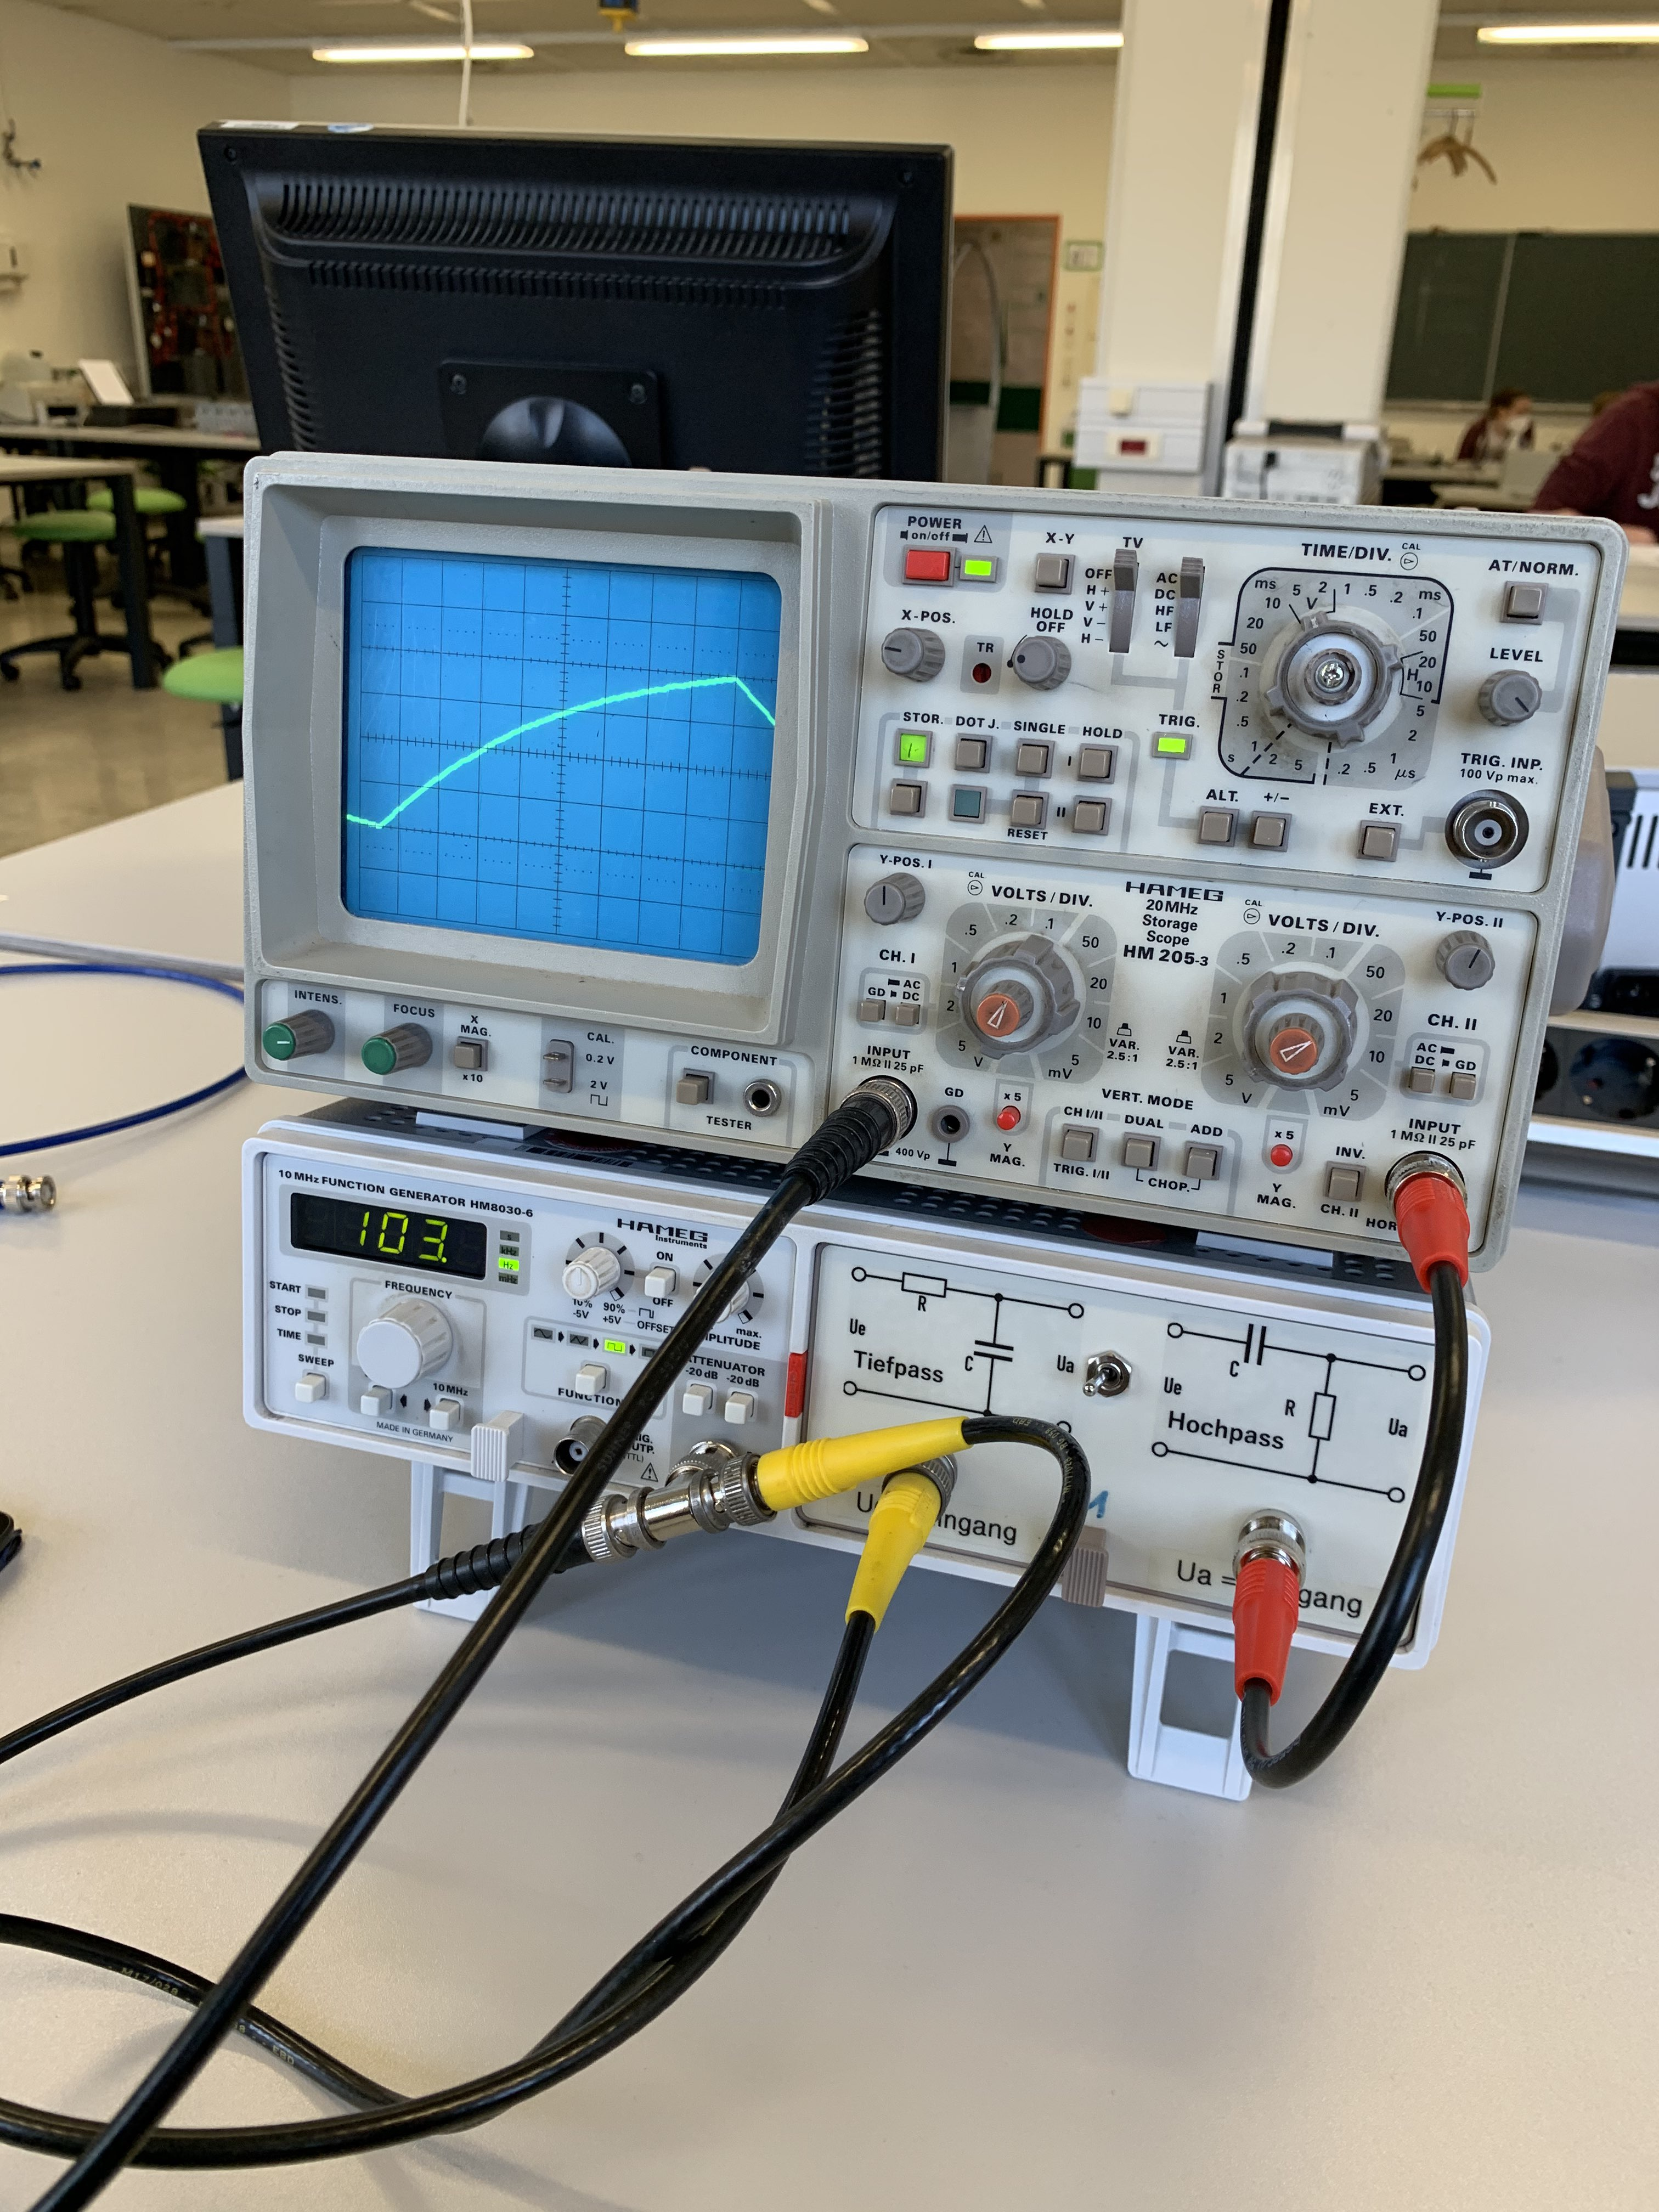
\includegraphics[scale=0.05]{bilder/oszillator.png}
        \caption{Oszillator.}
        \label{fig:aufbau}          
\end{wrapfigure}

Grundlegend wir der Versuch an einem Oszillator ausgeführt.
Dafür wird insbesondere ein Generator gebraucht, der in der Lage ist Spannungen verschiedener 
Typen herzustellen. Hier beschränken wir uns auf eine Rechteck - und Sinusspannung. 
Vom Oszillator soll dann jeweils die unmittelbare Spannung gemessen werden und die, 
die durch einen Kondensator und Widerstand modifiziert wurde.
Auf dem Display sieht man also sowohl die eingehende (Rechteck/ - Sinusspannung) als 
auch die ausgehende Spannung, also die Darstellung des Lade - und Entladungsevorgang des Kondensators.

%\vspace{1cm}
\section{Durchführung}
Die Durchführung teilt sich in die  drei folgenden Konfigurationen auf.
\subsection{Bestimmung der Zeitkonstante}
Um das Maß für die Geschwindigkeit zu errechnen gilt es also die Konstante $\text{RC}$ zu finden.
Dafür wird eine Rechtecksspannung vom Generator angelegt und am Oszillator das Laden beziehungsweise Entladen des
Kondensators beobachtet. In Intervallen von $\Delta t = \SI{2.5}{ms}$ wird der Strom $U_c$ abgelesen und die
Daten in eine Tabelle aufgenommen. 
\begin{figure}
    \centering
    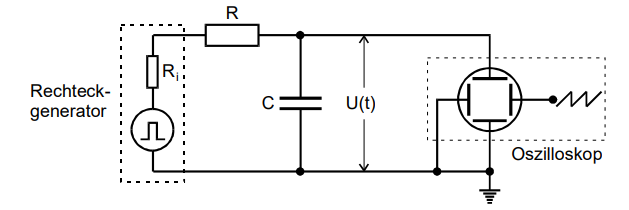
\includegraphics[width=\textwidth]{bilder/RC.png}
    \caption{Schaltplan zur Bestimmung der Zeitkonstanten.\cite{skript}}
    \label{fig:RC}
\end{figure}

\subsection{Amplitudenbestimmung der Kondensatorspannung}
\label{sectionref}
Nun wird eine Sinusspannung vom Generator erzeugt mit einer Frequenz, die im Laufe jeweils um einen Wert
von $\Delta \text{f}= \SI{500}{\hertz}$ angehoben wird. Die entsprechende Amplitude $U_c$ wird 
dem Oszillator entnommen und in eine Tabelle eingetragen.
 \begin{figure}
    \centering
    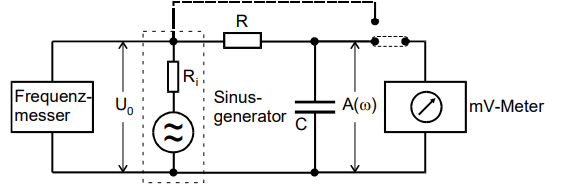
\includegraphics[width=\textwidth]{bilder/amplitude.png}
    \caption{Schaltplan zur Bestimmung der Frequenzabhängigkeit der Kondensatorspannungsamplitude.\cite{skript}}
    \label{fig:amp}
\end{figure}


\subsection{Messung der Phasenverschiebung}
Bei Beibehaltung der aktuellen Konfiguration wird der Vorgang aus \ref{sectionref} in gleichen Intervallen
wiederholt. Dabei werden beide Spannungen, die Eingehende und Ausgehende, angezeigt und achsensymetrisch
zur X - Achse ausgerichtet.\\
\begin{figure}
    \centering 
    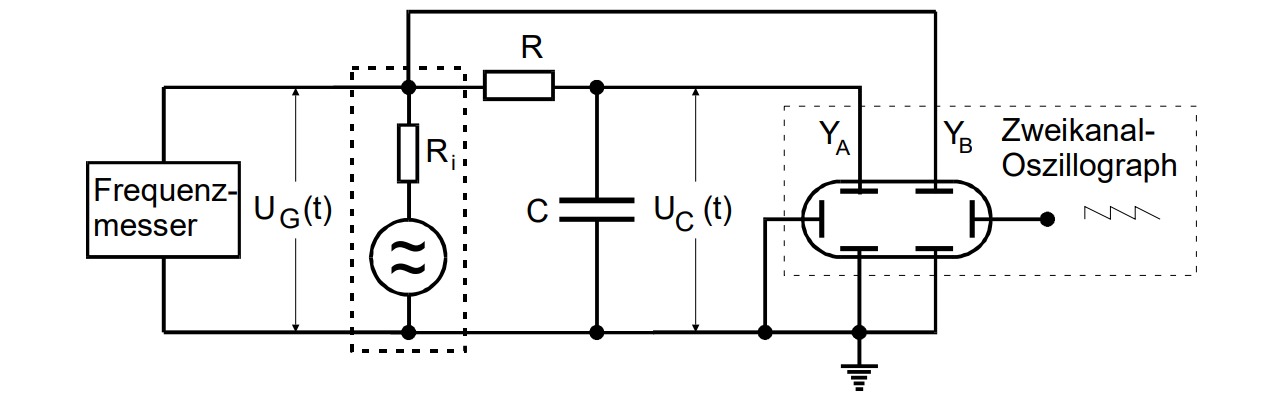
\includegraphics[width=\textwidth]{bilder/jetzt.png}
    \caption{Schaltplan zur Bestimmung der Phasenverschiebung zwischen zwei Spannungen.\cite{skript}}
    \label{fig:ab}
\end{figure} 
Ein nun messbarer Abstand $a$ und $b$ %ref zur darstlellung
ist bei entsprechender Frequenz und Amplitude zu entnehmen. Hier bildet $b$ eben die Wellenlänge
der Spannung $U_g$ ab. Die Phasenverschiebung $\phi$ resultiert aus folgender Gleichung.
\begin{equation}
    \label{eqn:phi}
    \phi= \frac{a}{b} \cdot 2 \pi
\end{equation}

\begin{figure}
    \centering
    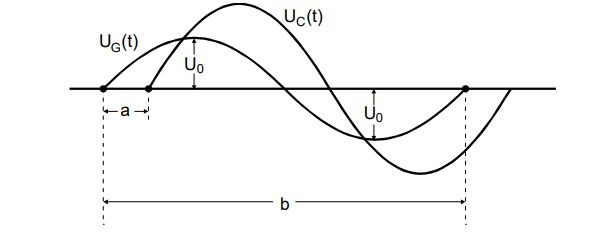
\includegraphics[width=\textwidth]{bilder/ab2.png}
    \caption{Art der Ablesung von Paramter $a$ und $b$.\cite{skript}}
    \label{fig:ab}
\end{figure}
